\section{Introduction}

Par la diversité des milieux qu'elle abrite, la chaîne des Alpes est une zone géographique propice à une grande biodiversité.
 Cet ensemble de massifs et de vallées constitue donc un laboratoire parfait pour étudier l'évolution des organismes dont les aires de répartitions semblent aisément observables.
\todo[inline]{Pas clair: pourquoi c'est facilement observable? Parce que c'est des patch d'habitat discrets?} 
 Cependant, l'histoire de cette orogenèse et les différents cycles glaciaires qui ont joué sur l'Holarctique complexifient énormément ces histoires biologiques.
 Ainsi, l'isolement géographique propice au processus de spéciation, ou encore l'adaptation à de nouvelles niches écologiques se sont trouvés modifiés de nombreuses fois par ces facteurs abiotiques.
 Ces nombreuses modifications ont aboutit à un état actuel de biodiversité où il est difficile de séparer ces ensembles de mécanismes, et conclure à une histoire biogéographique simple.
 En conséquence, on observe nombre d'espèces cryptiques, ou d'entités taxonomiques définies sur des critères évoluant rapidement dans la littérature.
 \todo[inline,caption={intro propre}]{Il faudrait réorganiser cette section. Introduire les espèces cryptiques est une très bonne idée, mais il faudrait expliquer pourquoi on en a pas mal dans la flore des Alpes. Pour l'instant on ne voit pas trop le lien.}

Dans le cadre de cette étude, il a donc été proposé d'approfondir l'étude de la structure génétique d'un groupe de plantes d'altitude : \textit{Primula} sect. \textit{Auricula} Scott subsect. \textit{Erythrodrosum} Pax. 
 Lors de récentes études phylogénétiques au niveau de la section \textit{Auricula} \citep{Zhang2004,Zhang2004a, Boucher2016a}, cette sous-section a été restructurée en s'appuyant sur des données génétiques nucléaires.
 Cependant la dernière étude de \citet{Boucher2016a} basée sur une nouvelle méthode de séquençage haut débit (hyRAD) suggère qu'un ensemble d'espèces ( \textit{P. apennina, P. cottia, P. pedemontana}) soit regroupé en une seule entité taxonomique, nommée ci-dessous \textit{P. pedemontana s.l.}.
 Cette proposition vient également soulever l'hypothèse d'une nouvelle sous-espèce à cette entité dans le massif des Écrins, qui pourrais être un hybride entre \textit{P. hirsuta} et \textit{P. pedemontana}.
 Cette population des Écrins a longtemps été une difficulté taxonomique pour les botanistes (\url{http://www.ecrins-parcnational.fr/actualite/lenigme-de-la-primevere-du-valgaudemar}) et les dernières analyses ne la considèrent pas comme une espèce propre.
 
\begin{figure}[!ht]
    \centering
    %\missingfigure[figwidth=12cm,figheight= 5cm]{Carte de répartition}
    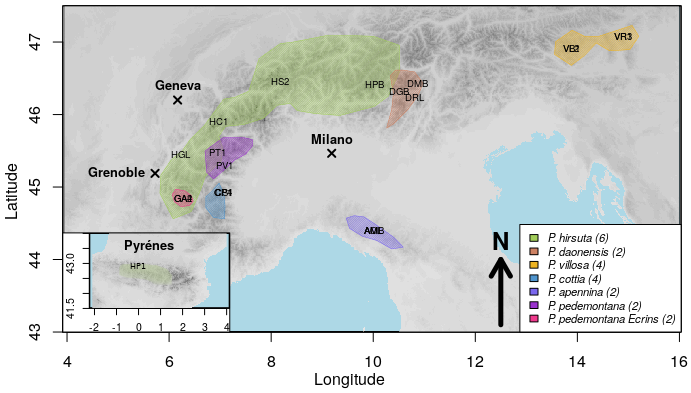
\includegraphics[width=0.9\textwidth]{fig/carte.png}
    \caption{\textbf{Carte de répartition de \textit{Primula} sect. \textit{Auricula} Scott subsect. \textit{Erythrodrosum} Pax.} Espèces composant la sous-section, avec entre parenthèse le nombre d'échantillons de cette étude. Les aires de répartitions sont extrapolées depuis les observations de l'INPN et du CBNA. Fond de carte : Température moyenne annuelle extraite de WorldClim. Résolution 30s (1km$^{2}$)}
    %http://worldclim.org/version2
    \label{carte}
    \centering
\end{figure} 
 
  \todo[inline,caption={intro trop détail}]{C'est trop de détails pour l'intro. il faut garder les détails taxonomiques/systématiques dans le premier paragraphe des méthodes. Ici ce qui compte à mon avis c'est de dire qu'on a un groupe d'espèces cryptiques et un taxon qu'on soupçonne d'être d'origine hybride. Pour être carré il faudra donner les noms d'auteurs des espèces que tu mentionnes, que tu trouveras dans la dernière révision taxonomique de Zhang et Kadereit.
  
De manière générale, je trouve cette intro un peu courte. Il faudrait essayer d'introduire les grandes questions de biogéographie et de biologie évolutive auxquelles ce sujet se rapporte. Du même coup ça permettrait d'expliquer pourquoi on s'intéresse à ce taxon en particulier. La section \textit{Auricula} n'est pas présentée non plus, alors que c'est le groupe de plantes le plus riche dans le système Alpin Européen (cf. papier d'Ozenda joint).}

Les buts de cette étude sont donc : (i) étudier le \clade{Hirsuta} à l'aide d'outils de génétique des populations; (ii) clarifier la structure de \textit{P. pedemontana s.l.}; (iii) étudier l'hypothèse d'hybridation/introgression du taxon des Écrins.

\todo[color=yellow]{intro review}

%%%%% intro de flo %%%%%%

%Déterminer quelles entités taxonomiques constituent des espèces distinctes est un des objectifs premier de la taxonomie mais est également d’une importance primordiale pour comprendre à la fois l’origine des espèces, le processus de spéciation, et leur futur probable, qui détermine les mesures de conservation qui sont éventuellement à prendre pour les protéger.
%	Si délimiter des espèces vivant en sympatrie est généralement une tâche facile, les complexes d’espèces cryptiques ayant des distributions allopatriques présentent souvent plus de difficulté (Coyne & Orr 2004). En effet, dans ces derniers cas les critères qui servent généralement à établir la présence d’isolement reproductif (absence de flux de gènes ou  d’individus hybrides entre lignées, etc.) ne peuvent pas être mesurés objectivement (Fujita et al. 2012). Pourtant, délimiter des espèces cryptiques distribuées en allopatrie permet d’étudier le rôle d’un des mécanismes de spéciation majeurs : l’isolement géographique (Mayr 1942). Dans certains cas où la dynamique de l’environnement abiotique au cours du temps est bien connue, de telles études permettent même de caractériser précisément l’influence de l’environnement sur la divergence évolutive entre lignées (Avise et al. 1987).

%	Dans le cadre de ce stage, nous tenterons de comprendre comment la dynamique du relief dans les Alpes (i.e. les phénomènes d’orogénèse, d’érosion et de glaciation) a contribué à la divergence d’espèces au sein d’un groupe de plantes de haute montagne : Primula sect. Auricula Scott subsect. Erythrodrosum Pax (ci-dessous, clade Hirsuta). Ce groupe comprend traditionnellement six espèces proches de P. hirsuta All. mais une étude récente a proposé de re-circonscrire P. pedemontana en fusionnant trois espèces, tout en suggérant qu’un taxon distinct existe dans le massif des Ecrins en France (Boucher et al. 2016). Nos objectifs de recherche seront les suivants :
%	1) Reconstruire les relations phylogénétiques entre taxons du clade Hirsuta et dater leurs divergences
%	2) Délimiter les taxons qui méritent le rang d’espèce au sein de ce clade et en particulier au sein du complexe de P. pedemontana s.l.
%	3) Comparer statistiquement différents scénarios afin de comprendre comment la dynamique des reliefs Alpins a influencé la divergence des espèces du clade Hirsuta

%	Pour cela, nous utiliserons des données de séquençage haut-débit obtenues grâce à la technique hyRAD (Suchan et al. 2016) . Ces données comprennent plusieurs milliers de SNPs indépendants pour 22 individus appartenant aux six espèces du clade Hirsuta actuellement reconnues (Boucher et al. 2016). Nous les analyserons d’abord avec des approches phylogénétiques standard comme le logiciel RAxML (Stamatakis 2014) et des avancées nouvelles permettant de dater des phylogénies inférées grâce à des SNPs (Stange et al. 2018). Afin de délimiter des espèces le plus objectivement possible à l’aide des données moléculaires disponibles, nous utiliserons la panoplie variée des techniques de la taxonomie moléculaire, incluant des techniques de clustering génétique mais aussi d’autre basées sur le coalescent (Fujita et al. 2012, Carstens et al. 2013, Leaché et al. 2014). Enfin, nous aurons recours à l’inférence ABC pour comparer explicitement différents scénarios de spéciation (Knwoles 2009, Cornuet et al. 2014).

%	Cette étude devrait nous aider à mieux comprendre l’influence de la dynamique du relief sur l’évolution de la flore des Alpes. Elle permettra également d’établir plus fermement le statut taxonomique du nouveau taxon de Primula découvert dans le massif des Ecrins, qui reste à ce jour un mystère (http://www.ecrins-parcnational.fr/actualite/lenigme-de-la-primevere-du-valgaudemar), et éventuellement d’envisager des mesures de conservation.